\documentclass{article}
\usepackage{graphicx} % Required for inserting images
\usepackage[top=0.9in, bottom=1in, left=1.5in, right=1.5in]{geometry}
\usepackage[utf8]{inputenc}
\usepackage[icelandic]{babel}
\usepackage[T1]{fontenc}
\usepackage[sc]{mathpazo}
\usepackage[parfill]{parskip}
\renewcommand{\baselinestretch}{1.2}
% Tables and lists
\usepackage{booktabs,tabularx}
\usepackage{multirow}
\usepackage{enumerate}
\usepackage{adjustbox}
\usepackage{multicol}
\usepackage{xcolor}
\usepackage{algpseudocode}
\usepackage{tikz}
\usepackage{nicefrac}
\usepackage{changepage}
\usetikzlibrary{arrows, positioning, calc, graphs}

% Math
\usepackage{amsmath, amsfonts, amssymb, amsthm}
% Graphics

\usepackage{graphicx}
\usepackage{tikz}
% Code environment
\usepackage{minted}
%\usepackage{bm}
%\usepackage{siunitx}
%\usepackage{animate}
%\usepackage{hyperref}
%\usepackage{movie15}
%\usepackage{multicol}
%\usepackage{changepage}
\title{Forritunarmál Hópverkefni 7}
\author{Ragnar Björn Ingvarsson, rbi3 \\
		Daníel Snær Halldórsson, dsh11 \\
		Ólafur Sær Sigursteinsson, oss27 \\
		Egill Askur Eineborg, eae28 \\
		Eygló Ástþórsdóttir, eya19 \\
		Elías Ver Bjarnason, evb17 \\
		Helga Björg Helgadóttir, hbh54 \\
		Máni Sverrisson, mas176 \\
		Yi Hu, yih2 \\
		Dagmar Ýr Eyþórsdóttir, dye2 \\
		Ana Margarida Delgado Costa, amd16}
\tikzset{->, >=stealth', shorten >=1pt, node distance=2cm,thick, main node/.style={circle,draw,minimum size=3em}}

\begin{document}
\renewcommand\thepage{}
	
	\maketitle

	\newpage
	\setcounter{page}{1}
	\renewcommand\thepage{\arabic{page}}

	\section{}
	\begin{verbatim}
;;;Notkun: mapreduce(f, op, u, x)
;;;Fyrir: f er einundarfall sem tekur við gildi af gerð a og
;;;       skilar gildi af gerð b, 
;;;       op er tvíundaraðgerð sem tekur inn tvö gildi, bæði
;;;       af gerð b og skilar gildi af gerð b.
;;;       u er gildi af gerð b og x er listi, [x1,x2,..,xn] af 
;;;       gildum af gerð a.
;;;Gildi: u op f(x1) op ... op f(xn) 
rec fun mapreduce(f, op, u, x)
{
    if (x==[])
    {
        return u;
    };
    return mapreduce(f, op, op(u, f(head(x))), tail(x));
};
	\end{verbatim}
	\begin{center}
		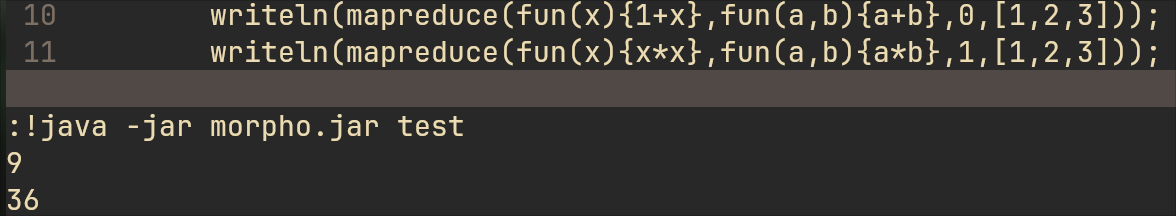
\includegraphics[scale=0.35]{mapreduce.png}
	\end{center}
	
	\newpage
	\section{}
	\begin{verbatim}
;;;Notkun: fromTo(i, j)
;;;Fyrir: i og j eru heiltölur, i<=j
;;;Gildi: Listinn [i,i+1,...,j-1]
rec fun fromTo(i, j)
{
    if (i == j)
    {
        return [];
    };
    return i : fromTo(i+1, j);
};
	\end{verbatim}
	\begin{center}
		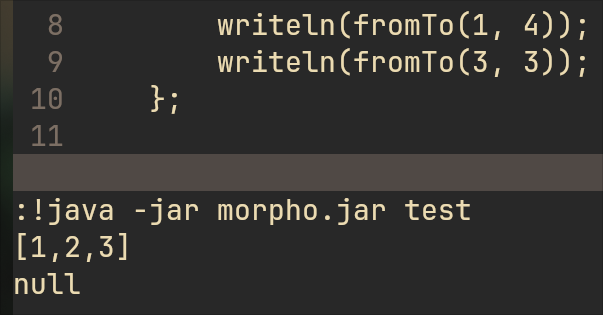
\includegraphics[scale=0.35]{fromto.png}
	\end{center}
	Ath. að þegar morpho prentar tóman lista þá prentast null gildið. Svo 
	fromTo(3,3) er í raun tómi listinn [].

	\newpage
	\section{}
	\begin{verbatim}
;;;Notkun: insertAt(x, i, z)
;;;Fyrir: x=[x1,x2,...,xN] er listi gilda af gerð a.
;;;       z er gildi af gerð a, i er heiltala, 0 <= i <= N
;;;Gildi: Listinn [x1,x2,...,x_i,z,x_(i+1),...,xN]
rec fun insertAt(x, i, z)
{
    if (i==0)
    {
        return z : insertAt(x, i-1, z);
    };
    if (x==[])
    {
        return [];
    };
    return head(x) : insertAt(tail(x), i-1, z);
};
	\end{verbatim}
	\begin{center}
		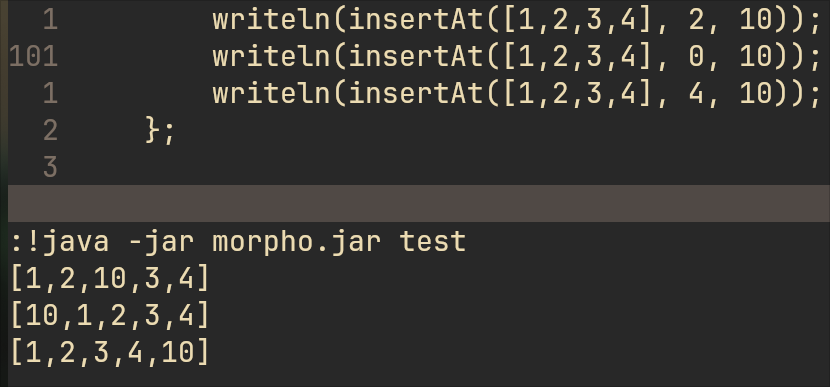
\includegraphics[scale=0.35]{insertat.png}
	\end{center}

	\newpage
	\section{}
	\begin{verbatim}
;;;Notkun: extendPermutation(n, z)
;;;Fyrir:  n >= 1 er heiltala.
;;;        z er einhver umröðun listans [1,2,...,n-1].
;;;Gildi:  Listi allra þeirra lista sem út koma þegar
;;;        tölunni n er skeytt inn í listann z á
;;;        einhverjum stað, allt frá byrjun til enda.
rec fun extendPermutation(n, z)
{
    if (z==[])
    {
        return [[n]];
    };
    return (n : z) : (map((fun(l){head(z) : l}), extendPermutation(n, tail(z))));
};
;;;Notkun: permutations(n)
;;;Fyrir:  n>=0 er heiltala.
;;;Gildi:  Listi allra umraðana listans [1,2,...,n].
rec fun permutations(n)
{
    if (n==0)
    {
        return [[]];
    };
    return mapreduce(
        fun(a){extendPermutation(n,a)},
        fun(a,b){a ++ b},
        [],
        permutations(n-1));
};
	\end{verbatim}
	\begin{center}
		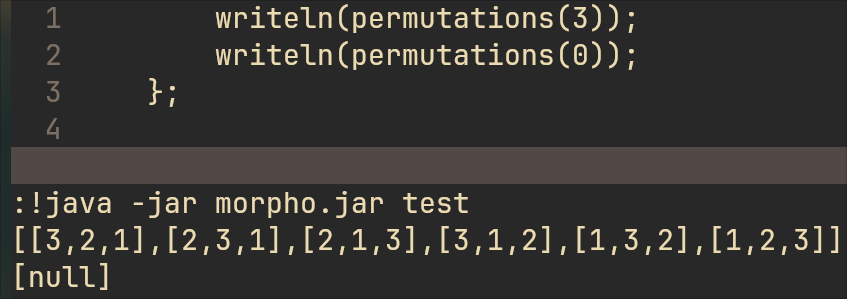
\includegraphics[scale=0.35]{permutations.png}
	\end{center}
	Ath. að þegar morpho prentar tóma listann prentast null gildið. Svo 
	permutations(0) er í raun [[]].

\end{document}
